\section{Results}
\label{sec:results}

Prices are for the 30 highest-ranked targets of each board against each rule's own leader unless stated, with cluster-bootstrap intervals (\Cref{sec:data}). ``Ceilings'' means the per-task boost is limited only by the task ceiling ($B\to\infty$).

\subsection{The price map: total boost is where the rules differ most}
\label{sec:pricemap}

\Cref{tab:price} gives the price of first place for each rule and board. With boosts limited only by ceilings, first place is feasible for every target under every rule, and the boost needed differs by a factor of 7 to 19 between the mean and the cheapest rule on each board. We report medians over the targets that are not already first under the rule (at most two per board and rule), because the others price at zero. The mean family is the expensive one: on HELM the median total boost is 360 points for the mean against 19 for plurality, 26 for the minimum and 36 for the median rule; on the Open LLM Leaderboard at sub-task level 134 against 10 for the median rule and 82 for plurality; at benchmark level 32 against 5 to 23 for the other rules. This follows \Cref{prop:mean}: the total boost under a mean is $m$ times the gap however it is spread, whereas the order and majority rules need a level on some tasks and nothing more. The mean's breadth is small: at ceilings it closes its gap on a median of 16\% of the HELM subjects, against two thirds for Copeland.

Targeting pays most for the rules that reward it (\Cref{fig:map}, Appendix~\ref{app:figs}): on HELM the depth of the cheapest uniform plan over that of the cheapest targeted plan is 1 for the mean by construction and 9 to 20 for plurality, median and minimum.

\begin{table}[t]
\centering
\caption{Price of first place at ceilings (medians over the 30 highest-ranked targets not yet first, own leader): total boost in points, breadth fraction $k/m$ and minimal feasible per-task budget $B^\ast$ in points. $\dagger$: some solver runs did not close (gap above $10^{-4}$); the cell is an upper bound.}
\label{tab:price}
\footnotesize\setlength{\tabcolsep}{3.5pt}
\begin{tabular}{@{}lrrrrrrrrr@{}}
\toprule
 & \multicolumn{3}{c}{HELM MMLU ($m{=}57$)} & \multicolumn{3}{c}{OLLB benchmarks ($m{=}6$)} & \multicolumn{3}{c}{OLLB sub-tasks ($m{=}39$)}\\
\cmidrule(lr){2-4}\cmidrule(lr){5-7}\cmidrule(lr){8-10}
Rule & boost & $k/m$ & $B^\ast$ & boost & $k/m$ & $B^\ast$ & boost & $k/m$ & $B^\ast$\\
\midrule
mean & 360 & 0.16 & 6.5 & 32 & 0.17 & 5.3 & 134 & 0.05 & 3.5\\
z-mean & 223 & 0.12 & 5.8 & 23 & 0.17 & 7.3 & 111 & 0.05 & 7.2\\
median & 36 & 0.20 & 4.9 & 5 & 0.17 & 2.4 & 10 & 0.13 & 5.1\\
min & 26 & 0.09 & 11.5 & 8 & 0.33 & 5.1 & 20 & 0.08 & 9.9\\
Borda & 222 & 0.58 & 6.0 & 9 & 0.17 & 3.6 & 26$^\dagger$ & 0.10 & 2.0\\
plurality & 19 & 0.12 & 2.7 & 17 & 0.33 & 9.2 & 82 & 0.21 & 11.9\\
Copeland & 98 & 0.67 & 4.6 & 7 & 0.33 & 3.7 & 33$^\dagger$ & 0.51 & 7.3\\
\bottomrule
\end{tabular}
% source: \texttt{results/price_magnitude.csv}, \texttt{results/price.csv}

\end{table}

\subsection{No rule is cheapest for every target}
\label{sec:nodominance}

No rule is cheapest in total boost for 90\% of the targets on any board (R2 holds, \Cref{tab:verdicts}). At a budget of 5 points the cheapest rule is plurality on HELM (for 73\% of targets, counting ties for every tied rule), the median on the benchmark-level board (53\%) and Borda on the sub-task board (67\%). The mean is the exception: at ceilings, against rules outside the mean family, it is the cheaper of two rules for at most 3\% of targets on HELM and the sub-task board and 13\% on the benchmark-level board. Against a common incumbent set the ordering on HELM is unchanged; on the Open LLM Leaderboard the minimum and Copeland move up.

\subsection{Breadth and the number of tasks}
\label{sec:breadth}

The pre-registered expectation was that median, plurality and Copeland need more breadth than the mean family. It fails on HELM, where it is reversed (R1; \Cref{tab:verdicts}): the median needs more breadth than the mean for 4\% of targets, plurality for 4\% and Copeland for 28\%, with paired differences in $k/m$ of $-0.43$, $-0.69$ and $-0.08$, all with intervals below zero. On the Open LLM Leaderboard it holds in part: at benchmark level the median (69\% of targets) and plurality (66\%) need more breadth and Copeland does not (38\%); at sub-task level plurality and Copeland need more for all targets and the median for 48\%. The test is made at the median minimal feasible budget of the mean family; other budgets are in \Cref{fig:paired} (Appendix~\ref{app:figs}).

\paragraph{Why the ordering flips.}
This account is post hoc and does not treat Copeland. At the common budget $b$ (0.55 to 0.65 standard deviations per task) the flip is one of feasibility. Plurality must win tasks outright, each costing the gap to the best score on it; the median largest such gap is 0.58 standard deviations on HELM, 1.20 at benchmark level and 2.56 at sub-task level, so plurality is feasible at $b$ for all targets on HELM but for only 20\% and 7\% on the other boards. An infeasible plan counts as breadth 1, which fixes the sign of the difference between plurality and the mean ($-0.84$, $+0.17$, $+0.77$ in $k/m$, medians over targets; R1 reports means). The mean is itself infeasible for 53\% of HELM targets; among targets feasible under both, the HELM advantage persists (median $-0.40$, plurality $-0.33$).

\paragraph{The crossing budget.}
The median needs less breadth than the mean below a crossing budget $B_\times$ and more above it. On HELM $B_\times$ is 2.8 standard deviations per task (interval 2.5 to 3.4, feasible plans only) and on the sub-task board 0.8 (0.7 to 0.9); for plurality on HELM and the median at benchmark level it does not exist on our grid, nor in depth anywhere.

Varying the number of tasks on the same models gives an answer that depends on the rule and the budget (\Cref{fig:m}). On random subsets of $m=5,\dots,57$ HELM subjects, the ratio of the breadth fraction of the median-type rules to that of the mean family falls with $\ln m$ at a budget of one task standard deviation (slope $-0.17$, interval $[-0.20,-0.14]$) and at two ($-0.06$, $[-0.10,-0.02]$) and rises at four ($+0.18$, $[0.14,0.23]$), so R4 fails at two. By rule, at two standard deviations the ratio for Copeland rises with $m$ (slope $+0.27$) while those for the median ($-0.15$) and plurality ($-0.30$) fall. On the same Open LLM Leaderboard models, going from bundled plans ($m=6$) to free sub-task plans ($m=39$) raises, at two standard deviations, Copeland's breadth ratio by $0.93$ ($[0.65,1.12]$) and lowers the median's by $0.66$ ($[-0.73,-0.62]$); plurality's change contains zero.

\begin{figure}[t]
\centering
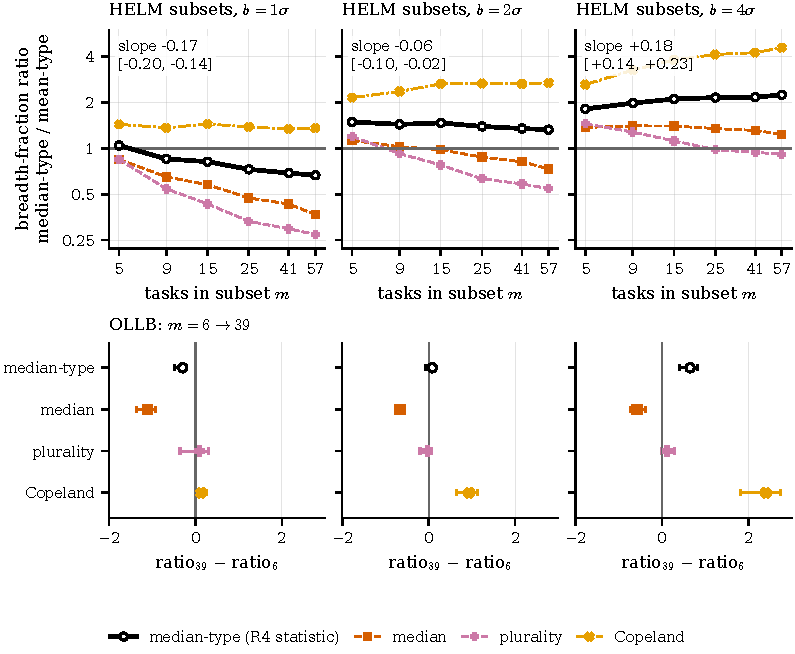
\includegraphics{../figures/fig3_m_effect.pdf}
\caption{Breadth-fraction ratio of the median-type rules to the mean family against the number of tasks $m$ (R4 predicts a rise). Top: random HELM subject subsets (same 79 models) at budgets of one, two (primary) and four task standard deviations; black: the R4 statistic with its slope against $\ln m$. Bottom: Open LLM Leaderboard, change in the ratio from bundled benchmark plans ($m=6$) to free sub-task plans ($m=39$), by rule. Infeasible cells count as breadth fraction 1.}
\label{fig:m}
\end{figure}

\subsection{What predicts the price}
\label{sec:predictors}

The pre-registered prediction R3 is that a rule's gap to the incumbent does not by itself carry the price from one board to another; it is borne out for all seven rules, since each fails in its worst direction (\Cref{tab:verdicts}). The pre-registered test is in raw units: the held-out $R^2$ of log price on the rule's own gap, fitted on one board and tested on another, is negative in the worst of the six directions for six of seven rules (the minimum's is 0.15), and in the best direction reaches 0.85 for the mean, 0.89 for the median and 0.93 for the minimum, and at most 0.24 for the others, so the gap carries the price of the minimum and the median in single directions only. Within a board, with families of models held out in turn, the gap predicts the price at ceilings with a cross-validated $R^2$ of 0.5 to 1.0 for every rule except plurality (0.0 to 0.65): the gap-to-price map is rule- and board-specific, not absent. The mean's failure is by construction (its depth is $m$ times the gap): per task its gap-only $R^2$ is 1.00, while the six other rules still do not transfer (worst direction $-2.9$ to $-1608$; \Cref{app:r3norm}).

We also tested, after R1 and R4 failed, whether summaries of the target's deficit profile (its Gini coefficient, the Lorenz share of its smaller half, the share of tasks within one standard deviation of the incumbent) add to the gap. Retention required a held-out gain of at least 0.1 in $R^2$ with an interval above zero. For the mean the gain is zero (the price is a function of the gap) and the z-mean never retains it. Within a board it holds for the minimum on HELM and at benchmark level and for plurality at benchmark level; across boards it holds in 11 of 122 cases with the intercept re-estimated (37 with the fitted intercept kept, where the gap-only baseline is far below zero). We take the hypothesis as not supported in general.

\subsection{Units, noise and the scale of a boost}
\label{sec:robustness}

\paragraph{Units.}
That the median-type rules are cheaper than the mean family under a cap does not survive a change of unit (R5; \Cref{tab:verdicts}): on HELM they are cheaper in points, in standard deviations and under a convex cost but not as a fraction of headroom; uncapped, they are cheaper in all four units on all boards.

\paragraph{Noise.}
Requiring the aggregate to lead by $c$ noise standard deviations, every top-30 target reaches a 90\% chance of first place under the mean family, the median and the minimum, on HELM and on the sub-task board. The depth at $c=0$ is multiplied by 1.2 to 2.0 for the mean family, 3.4 to 6.2 for the minimum and 6.2 to 6.7 for the median, and the median needs the widest margin ($c=8$ against 3 on HELM, 4 against 2 on the sub-task board; \Cref{app:e6e7}). The other rules were not run with noise.

\paragraph{Calibration of the boost scale.}\label{sec:calibration}
Open LLM Leaderboard fine-tunes with a base model on the board (498 pairs from 76 bases) show median best-task gains of 8 to 9 points for parents under 9B and 27 to 36 points for parents of 9B and above (\Cref{fig:calib}); the budgets that matter (median $B^\ast$ of 2 to 12 points, \Cref{tab:price}) lie within these gains only for parents of 9B and above. For the top targets (mostly 70B and above) and for HELM, which has no pairs, the scale is an assumption.

\begin{table}[t]
\centering
\caption{Pre-registered tests and verdicts, each against the direction predicted (S, P, F: supported, partial, failed). HELM-57 has $m=57$ subjects; OLLB-6 and OLLB-39 are the Open LLM Leaderboard at benchmark ($m=6$) and sub-task ($m=39$) level. The last three rows are exploratory and post hoc.}
\label{tab:verdicts}
\footnotesize\setlength{\tabcolsep}{2.5pt}
\begin{tabular}{@{}>{\raggedright\arraybackslash}p{0.58in}>{\raggedright\arraybackslash}p{0.82in}>{\raggedright\arraybackslash}p{3.2in}>{\raggedright\arraybackslash}p{0.7in}@{}}
\toprule
Scope & Value & 95\% CI / detail & Verdict\\
\midrule
\multicolumn{4}{@{}>{\raggedright\arraybackslash}p{5.4in}}{\emph{R1: median-type rules (median, plurality, Copeland) need more breadth than the mean. Share of targets ($\ge0.8$ predicted); paired difference in $k/m$ [95\% CI] ($>0$ predicted); S/P/F = supported/partial/failed}}\\
HELM-57 & 0.04/0.04/0.28 & $-$0.43\,[$-$0.57,$-$0.29]\hspace{2pt}$-$0.69\,[$-$0.77,$-$0.57]\hspace{2pt}$-$0.08\,[$-$0.12,$-$0.01] & F, F, F\\
OLLB-6 & 0.69/0.66/0.38 & 0.26\,[0.17,0.37]\hspace{2pt}0.22\,[0.16,0.38]\hspace{2pt}0.03\,[$-$0.10,0.14] & P, P, F\\
OLLB-39 & 0.48/1.00/1.00 & 0.08\,[$-$0.01,0.25]\hspace{2pt}0.72\,[0.66,0.86]\hspace{2pt}0.49\,[0.42,0.63] & F, S, S\\
\addlinespace[2pt]\multicolumn{4}{@{}>{\raggedright\arraybackslash}p{5.4in}}{\emph{R2: no rule is cheapest in depth for $\ge90\%$ of targets (largest share over budgets, incumbents)}}\\
each board & \multicolumn{2}{>{\raggedright\arraybackslash}p{4.09in}}{HELM-57 plurality 0.73; OLLB-6 median 0.53; OLLB-39 Borda 0.67} & supported\\
\addlinespace[2pt]\multicolumn{4}{@{}>{\raggedright\arraybackslash}p{5.4in}}{\emph{R3: the gap alone does not predict price (held-out $R^2<0.9$ in the worst of the six directions)}}\\
across & \multicolumn{2}{>{\raggedright\arraybackslash}p{4.09in}}{worst direction per rule: best 0.15, lowest $-1.3\times10^{3}$; $<0$ for 6 of 7} & supported\\
within & \multicolumn{2}{>{\raggedright\arraybackslash}p{4.09in}}{grouped-CV $R^2$ over target families: 0.50--1.00; plurality 0.00--0.65} & --\\
\addlinespace[2pt]\multicolumn{4}{@{}>{\raggedright\arraybackslash}p{5.4in}}{\emph{R4: median/mean breadth ratio rises with $m$ (slope $>0$ predicted; $b=2\sigma$, other $b$ in Fig.~\ref{fig:m})}}\\
HELM & slope vs $\ln m$ & $-$0.058 [$-$0.101, $-$0.018] & failed\\
OLLB & ratio$_{39}-$ratio$_{6}$ & 0.080 [$-$0.063, 0.152] & failed\\
\addlinespace[2pt]\multicolumn{4}{@{}>{\raggedright\arraybackslash}p{5.4in}}{\emph{R5: median-type cheaper in all 4 units and $\tau\ge0.5$: min Kendall $\tau$; units cheaper; cap/no cap; S/P/F}}\\
HELM-57 & 0.73/0.52 & median-type cheaper in 3/4 of 4 units & F/S\\
OLLB-6 & 0.40/0.33 & median-type cheaper in 0/4 of 4 units & P/P\\
OLLB-39 & 0.18/0.50 & median-type cheaper in 2/4 of 4 units & F/P\\
\addlinespace[2pt]\multicolumn{4}{@{}>{\raggedright\arraybackslash}p{5.4in}}{\emph{Crossing budget $B_\times$ ($\sigma$/task) above which the median needs more breadth than the mean (feasible; 95\% CI)}}\\
crossing & \multicolumn{2}{>{\raggedright\arraybackslash}p{4.09in}}{median: HELM-57 2.8 [2.5, 3.4]; OLLB-6 none; OLLB-39 0.8 [0.7, 0.9]; plurality: HELM-57 none} & --\\
\addlinespace[2pt]\multicolumn{4}{@{}>{\raggedright\arraybackslash}p{5.4in}}{\emph{Deficit-profile test (exploratory, post hoc): profile adds $\ge0.1$ held-out $R^2$ to the gap (CI above 0); cross-board, intercept re-estimated}}\\
profile & \multicolumn{2}{>{\raggedright\arraybackslash}p{4.09in}}{retained in 11 of 122 cases (37 with the fitted intercept kept): median 2, min 4, plurality 5; mean: gain 0 (identity); z-mean: never retained} & not supported\\
\bottomrule
\end{tabular}
% source: \texttt{results/verdicts.csv}, \texttt{results/predictors_within.csv}, \texttt{results/bx_crossing.csv}, \texttt{results/predictors_hl.csv}

\end{table}
